\chapter{\label{ch:ml}Neural Networks} 

\minitoc

Machine Learning (ML) is a field of research, which studies algorithms that
can learn to make predictions from data, i.e. predict a set of output variables,
given a set of input variables. The algorithms typically take the form of a
multivariate function, which is used to predict the output\cite{Reed1999}.

ML algorithms are often classified into four groups based on two distinctions: 
regression or classification, and supervised or unsupervised. The first
distinction is based on the nature of the output distribution expected from the
network; regression algorithms are designed to predict the outputs of a 
continuous function, whereas classification algorithms aim to separate data 
into groups. The distinction between supervised and unsupervised algorithms is 
based on the outputs used during training; in a supervised algorithm the true 
output is known, and the network's goal is to predict the true output, while 
in an unsupervised algorithm the output is unknown, and the networks goal is 
to extract meaningful structure from the data\cite{Lecun2015}.

Chapters \ref{ch:chargeid} and \ref{ch:michel} of this thesis describe two 
examples of the application of Neural Networks (NN) for event reconstruction 
in LArTPC data. These algorithms are classification algorithms based on the
supervised learning approach. This chapter will not provide a full survey of
the available ML techniques, which are both numerous and diverse. Instead it 
will briefly describe the theory behind NNs, as well as providing details of 
the techniques used in the subsequent chapters. 

\section{Artificial Neural Networks}
Artificial neural networks (ANN) are a class of ML algorithm that draw
inspiration from biological neurons. An ANN consists of a set of nodes, along
with a set of connections between those nodes. The set of nodes and connections
is often referred to as a graph or architecture. The nodes in 
the graph take the form of artificial neurons, which pass a number of inputs 
through an activation function to produce a single output, as depicted in 
Figure \ref{fig:neuron}.  The output of each neuron is either distributed to 
subsequent neurons in the network, or it is part of the output of the network. 
\begin{figure}

	\centering

	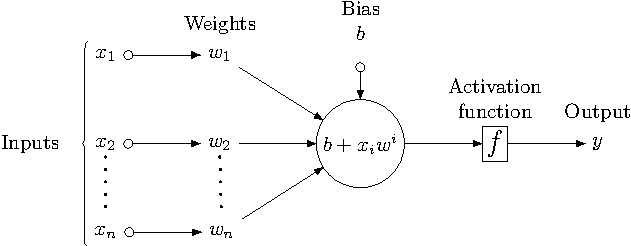
\includegraphics[width = 0.7\textwidth]{figures/neuron.pdf}

	\caption
	[Graphical representation of an individual neuron in an artificial neural
	network.]
	{Graphical representation of an individual neuron in an artificial neural
	network.}

	\label{fig:neuron}

\end{figure}

One of the most widely used ANNs is the multi--layer perceptron 
(MLP)\cite{Reed1999}; this class of network consists of at least three layers 
of nodes: an input layer, one or more hidden layers, and an output layer. The 
layers are connected in a feedforward configuration, such that the graph of 
nodes contains no cycles. The layers of an MLP are often fully connected or 
dense, meaning that the output of every node is connected to the input of 
every node in the next layer of the network. An example of a fully connected 
MLP, with two hidden layers, is shown in Figure \ref{fig:mlp}. 

\begin{figure}

	\centering

	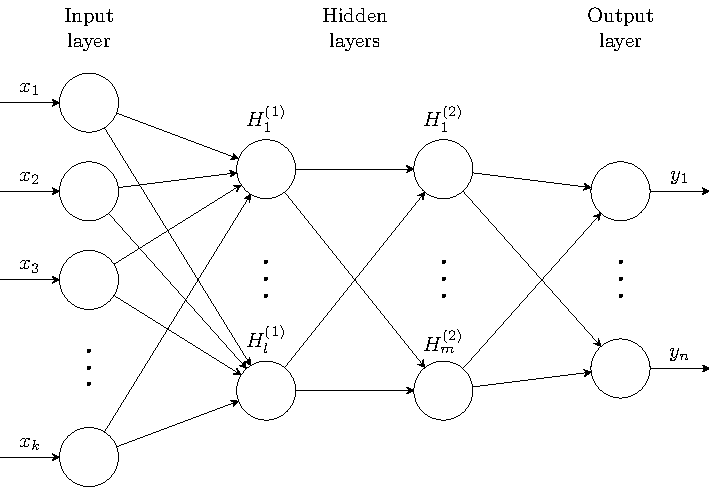
\includegraphics[width = 0.8\textwidth]{figures/mlp.pdf}

	\caption
	[A graphical representation of a multi--layer perceptron.]
	{ A graphical representation of a multi--layer perceptron. }

	\label{fig:mlp}

\end{figure}

Each node receives input from nodes in the previous layer, and uses the inputs
to calculate a response function. For the $i^{th}$ node in the $j^{th}$ layer 
of a network, 
\begin{equation*}
	a^{i,j} = \mathbf{w}^{i,j} \cdot \mathbf{x}^{j-1} + b^{i,j}
\end{equation*}
where $a^{i,j}$ is the response function, $\mathbf{w}^{i,j}$ is the weights
vector, $b^{i,j}$ is the bias, and $\mathbf{x}^{j-1}$ is the input vector from 
the previous layer. This response function is usually passed through a
nonlinear activation function, $f$, to produce the output from the node,
$y$, which is part of the input for the next layer,
\begin{equation*}
	\left(\mathbf{x}^j\right)_i = y^{i,j} = f \left( a^{i,j} \right).
\end{equation*}

Some common choices for the activation function are the sigmoid function, the
hyperbolic tangent, the rectified linear unit (ReLU), and the softmax 
function\cite{Lecun2015, He2015, Szegedy2015}.
\begin{align}
	\tag{Sigmoid} f(x) &= \frac{1}{1+e^x} \\
	\tag{Tanh}    f(x) &= \frac{e^x - e^{-x}}{e^x+e^{-x}} \\
	\tag{ReLU}    f(x) &= \mbox{max}\left( 0, x \right) \\
	\tag{Softmax} f(x_i) &= \frac{e^{x_i}}{\displaystyle\sum_j e^{x_j}} \\
	\label{eqn:losses}
\end{align}
In the softmax function, the index $i$ indicates the current node, and the index
$j$ includes all nodes in the current layer. This construction ensures that 
the outputs from a softmax layer sum to one, and as such this unit is commonly 
used in categorisation tasks when the output must belong to one of a given set 
of categories. The benefits and drawbacks of these common activation functions 
will be discussed later in this chapter, when we discuss modifying weights 
with the backpropagation algorithm.

The weights and biases of the nodes in an MLP can be adjusted to make accurate 
predictions of data. For a classification task, there are typically as many
output nodes as there are classes, with output values in the range zero to one. 
The output value of a classification network, quantifies how well the image
represents each class, based on the networks prediction. In principle, MLPs 
are able to approximate any function to arbitrary precision with a 
single hidden layer\cite{Cybenko1989ApproximationBS}; however, there is no 
limit on the number of nodes required in order to achieve a good 
approximation. In practice, networks with additional hidden layers can reach 
the required precision with fewer nodes than a network with a single hidden 
layer, but there are diminishing returns with more than a few hidden 
layers\cite{Reed1999, Lecun2015}.

\subsection{Convolutional Neural Networks}
An extension of the MLP with considerable success, particularly in image 
classification tasks, is the convolutional neural network 
(CNN)\cite{Jackel2008, Szegedy2015, 5537907}, which addresses some of the drawbacks 
of the traditional MLP. In particular, when evaluating data with a high 
dimensional input, having a fully connected network architecture leads to a 
large number of neurons and high computational cost. In addition, for 
spatially correlated data, such an architecture does not take into account the 
local spatial structure of the data, instead focussing on all the data at 
once. A CNN attempts to resolve these issues by exploiting the local spatial 
structure of the data.

In a CNN the singular input neutrons of a traditional MLP are replaced by
convolutional kernels. A convolutional kernel is a matrix containing a set of 
weights, which are multiplied pixel--by--pixel with small regions of the input 
image. The convolution operator is defined as, 
\begin{equation}
	\left( x * y \right)_i = \sum_{j = - \infty}^{\infty} x_j \; y_{i-j},
\end{equation}
where x and y are discrete sequences. In the machine learning context, y
represents the image, and x the convolutional kernel, which are both finite in
extent. Therefore, they are defined to be zero outside of their boundaries, and
the sum range can be reduced to $\left[0, N\right]$, where $N$ is the number 
of pixels in the kernel. The convolution operation is applied to all pixels in 
the input image, which are replaced by the resulting convolution in the next 
layer of the network. Many convolutional kernels are used in each layer of the 
network, each producing an output image which is passed to the next 
layer. 

Convolutional kernels are sometimes referred to as feature detectors, which 
emphasises the fact that each kernel identifies a given feature in the data, 
based on the weights in the kernel matrix. The output image from each kernel 
is known as a feature map, reflecting the fact that they represent the spatial 
distribution of the features learned by a given feature detector. An example of
a commonly used feature detector and the output feature map is given in Figure
\ref{fig:edge_detector}. This feature map is the result of applying a Sobel edge
detector\cite{kanopoulos1988design} to the input image.
\begin{figure}

	\centering

	\begin{subfigure}[b]{0.49\textwidth}
		\centering
		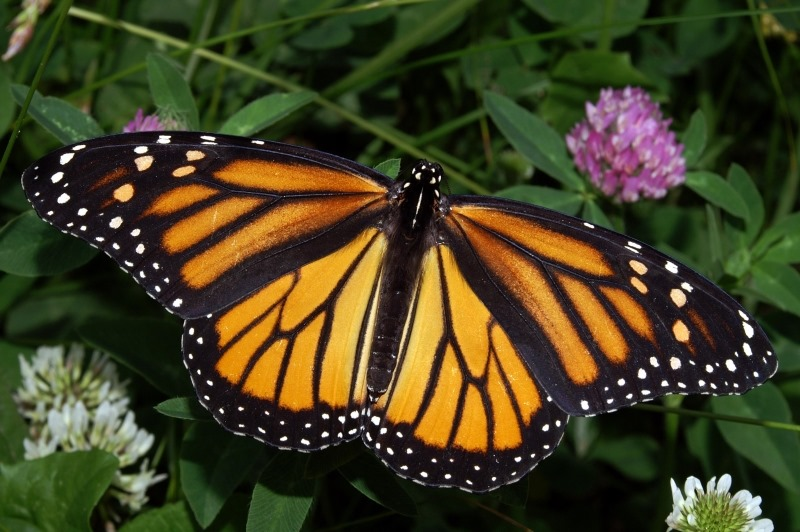
\includegraphics[width=\textwidth]{figures/ed_input.jpg}
		\caption{Input Image.}
		\label{fig:ed_input}
	\end{subfigure}
	\hfill
	\begin{subfigure}[b]{0.49\textwidth}
		\centering
		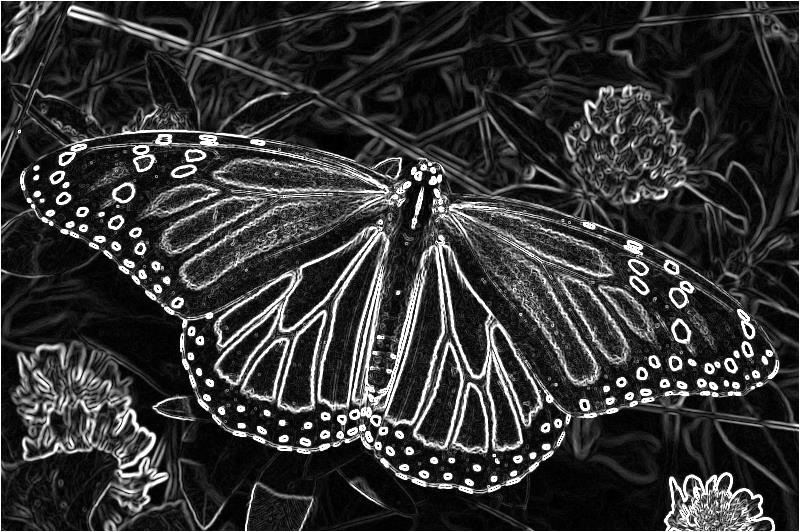
\includegraphics[width=\textwidth]{figures/ed_feature_map.jpg}
		\caption{Feature Map.}
		\label{fig:ed_feature_map}
	\end{subfigure}

	\caption
	[Application of a Sobel edge detector to an image.]
	{Application of a Sobel edge detector to an image. Images from
	\cite{edge_detector}.}

	\label{fig:edge_detector}

\end{figure}

\subsubsection*{Pooling}
The use of images as network input typically drastically increases the number of
input parameters for a network, when combined with a large number of
convolutional filters this can lead to a dramatic increase in the computational
cost of training a network. Pooling\cite{5537907} is a downsampling technique 
designed to reduce the number of parameters in the network and ,therefore, 
reduce the computational cost of making predictions. In pooling algorithms
the data from each $m \times n$ region of the input is downsampled to a single 
value, the downsampled image is used as the input for the next layer of the 
network. Two common pooling algorithms are max pooling and average pooling; in 
max pooling the maximum value from within the downsampling region is used, 
whereas average pooling uses the average value from the region.

\bigskip
\noindent
While convolutions are able to extract features from the data, they typically
are not able to make predictions in the desired format for classification tasks.
Therefore, after convolutions, data is typically flattened and passed through
one or more dense layers in order to produce the classification prediction. A
graphical representation of a typical CNN architecture is shown in Figure
\ref{fig:cnn_layer}, it includes convolutional, pooling, and dense layers.
\begin{figure}
	\centering
	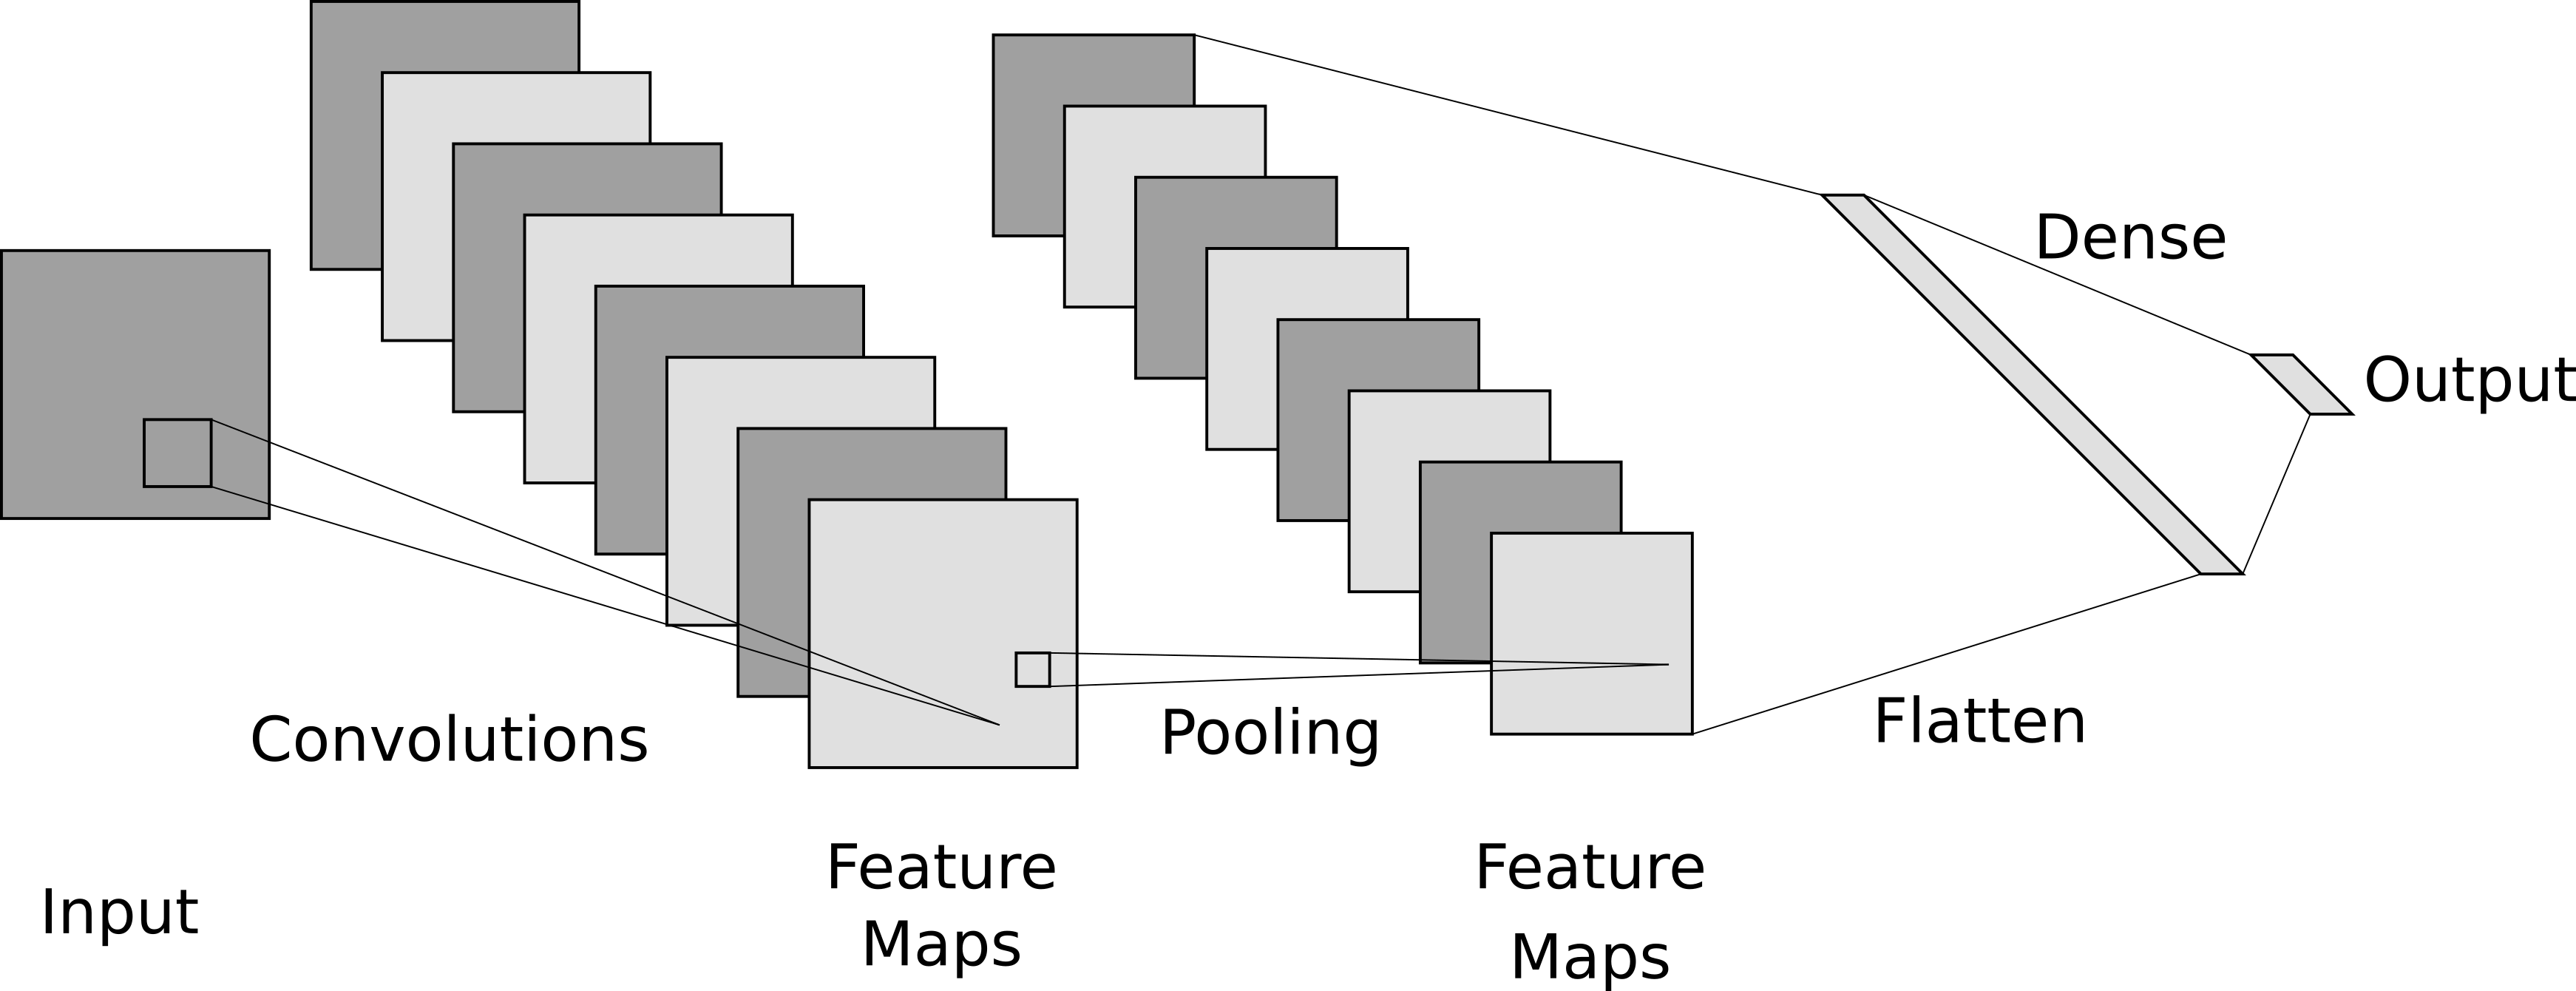
\includegraphics[width = \textwidth]{figures/cnn_layer.png}
	\caption
	[A graphical representation of a convolutional neural network.]
	{ A graphical representation of a convolutional neural network. Figure
	generated with \cite{cnn_diagrams}.}
	\label{fig:cnn_layer}
\end{figure}

\subsection{Residual Neural Networks}
Adding more layers to a neural network usually improves the performance, the
popular intuition for this is that with each subsequent layer the network is
able to learn more complex features of the image with which to make it's
classification. In fact, adding more layers should never decrease the 
performance of a network, because the new layers could be set to be the 
identity, which would result in the same output from the network. However, it 
has been demonstrated that adding too many layers to a simple neural network 
will reduce performance, suggesting that the optimisation of
larger networks leads to degradation\cite{He_2016_CVPR}.

One method which has been shown to counter the degradation of deep networks, 
is the use of residual neural networks (ResNet). In a ResNet, the input to 
each layer is combined with the results of the convolutions as part of the 
input to a future layer; in effect, the identity transformation has been added
to the set of operations in the layer. An example of these shortcut connections 
is shown in Figure \ref{fig:short_connect}\cite{He_2016_CVPR}. 
\begin{figure}
	\centering
	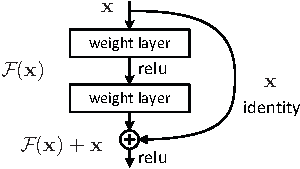
\includegraphics[width = 0.6\textwidth]{figures/short_connect.pdf}
	\caption
	[An example of a shortcut connection in a convolutional neural network.]
	{An example of a shortcut connection in a convolutional neural network.
	Figure from \cite{He_2016_CVPR}.}
	\label{fig:short_connect}
\end{figure}

\section{Supervised Learning}
Supervised learning is the process of teaching a neural network to accurately
predict the correct output, the ground truth, for a given input. The network is 
optimised by minimising the loss function, which quantifies the difference 
between the network output and the ground truth. The choice of loss function 
is dependent on the problem being considered, specific examples will be 
discussed in subsequent chapters, which will detail the CNN algorithms 
developed as part of this thesis.

The output of a neural network, g(x), is the result of a chain of function 
evaluations and matrix multiplication; for a network with $n$ layers,
\begin{equation*}
	g(x) = f^n(W^n f^{n-1}(W^{n-1} \;...\; f^1(W^1 x) \;...\; ).
\end{equation*}
where $g$ is the output of the network, $x$ is the input, $f$ are the 
activation functions for each layer, and $W$ are the weights for each layer. 
The loss of the network is given by the loss function, L,  evaluated on the 
output of the network and the ground truth, y,
\begin{equation*}
	L(y, g(x)).
\end{equation*}

To make accurate predictions with a NN, quantified by the loss function, the
weights and biases of the network need to be optimised. The backpropagation
algorithm\cite{Rumelhart1986} is currently the most widely used algorithm for
minimising the loss function by adjusting the weights and biases in the network.

Consider the weight for the $j^{th}$ node in the $l^{th}$ layer of a network for
and incoming connection from the $i^{th}$ node from the previous layer, 
$W^l_{ij}$, the loss function varies with respect to these weights as 
$\partial L/\partial W^l_{ ij }$. If we modify the weights with, 
\begin{equation} 
	\Delta W^l_{ ij } = -\eta \frac{\partial L}{\partial W^l_{ ij }},
	\label{eq:delta_w}
\end{equation}
for positive learning rates, $\eta > 0$, we are guaranteed to reduce the loss
for a given input. The backpropagation algorithm provides an algorithm for 
calculating the derivatives required to adjust the weights in each layer.

Applying the chain rule to the right hand side of Equation \ref{eq:delta_w},
\begin{equation}
	\frac{\partial L}{\partial W^l_{ij}} = \frac{\partial L}{\partial a^l_j} \;
	\frac{\partial a^l_j}{\partial W^l_{ij}},
	\label{eq:backprop_chain_rule}
\end{equation}
where $a^l$ are response functions for the nodes in layer $l$. The derivative 
of the response function with respect to the weights, is just the input from the
previous layer,
\begin{equation}
	\frac{\partial a^l_j}{\partial W^l_{ij}} = \frac{\partial}{\partial W^l_{ij}}
	\left( \sum_{k = 1}^{n_l} W^l_{kj} x^{l-1}_{k} \right) = x^{l-1}_i,
	\label{eq:backprop_d_activ}
\end{equation}
where $x^{l-1}$ are the outputs from layer $l-1$, and $n_l$ is the number of 
nodes in layer $l$. The other term, which is often denoted as $\delta^l_j$, is 
known as the error; this term will be discussed shortly. Combining Equations 
\ref{eq:backprop_chain_rule} and \ref{eq:backprop_d_activ} gives,
\begin{equation*}
	\frac{\partial L}{\partial W^l_{ij}} = \delta^l_j \; x^{l-1}_i.
\end{equation*}

The value of the error depends on the loss function being used in each 
particular model. The error can also be shown to have a recursive relationship 
via the chain rule,
\begin{align*}
		\delta^l_j = \frac{\partial L}{\partial a^l_j} &= \sum_{k=1}^{n^{l+1}} 
		\frac{\partial L}{\partial a^{l+1}_{k}}\frac{\partial a^{l+1}_k}{\partial 
		a^l_j}\\ 
		&= \sum^{n^{l+1}}_{k = 1} \delta^{l+1}_k \frac{\partial a^{l+1}_k}{\partial 
		a^l_j},
\end{align*}
where the sum is over all nodes in layer $l+1$. We can use the definition of the
response function to simplify this further,
\begin{align*}
		\frac{\partial a^{l+1}_k}{\partial a^l_j} &= \frac{\partial}{\partial a^l_j} 
		\left( \sum^{n^l}_{p=1} W^{l+1}_{pk} f(a^l_p) \right) \\ 
		&= W^{l+1}_{jk} \; f^\prime(a^l_j)
\end{align*}
where $f$ is the activation function. The error is, therefore,
\begin{equation*}
	\delta^l_j = \sum^{n^{l+1}}_{k=1} \delta^{l+1}_k W^{l+1}_{jk} f^\prime(a^l_j),
\end{equation*}
which depends on the value of the error in the following layer.

Based on these manipulations with the chain rule, the backpropagation 
algorithm is as follows,
\begin{enumerate}
	\item Calculate the forward pass, while storing the results for $g(x)$, 
		$a^l_j$, and $x^l_j$.
	\item Starting at the output layer, calculate the derivatives, going backwards
		through the network. 
	\begin{itemize}
		\item Store the results for $\delta^l_j$, to use when calculating subsequent
			layers.
	\end{itemize}
	\item Update the weights according to the update rule in Equation 
		\ref{eq:delta_w}.
\end{enumerate}

The backpropagation algorithm is used to calculate the gradients in order to
adjust weights in a neural network. There are a number of optimisation 
algorithms for adjusting the weights, such as mini--batch stochastic gradient 
descent (SGD)\cite{10.1145/2623330.2623612}, and Adaptive Momentum Estimation 
(Adam)\cite{KingmaD.P.2015AAMf}. The details of these algorithms are not 
important for the discussion in this thesis and, therefore, they will only be 
mentioned in passing here, a review of gradient descent optimisation 
algorithms can be found here \cite{ruder2016overview}. Some methodologies are
common among many optimisation techniques, three important examples are the 
ideas of mini--batches, training iterations, and training epochs. A mini--batch
is a small sample of the input data, on which the backpropagation algorithm is
applied simultaneously, this corresponds to one training iteration. A training
epoch, which consists of a number of training iterations, refers to one cycle
through the full training dataset, such that the network has been trained on 
every training example exactly once.

\bigskip
\noindent
The rate of learning in the backpropagation algorithm is dependent on the
derivative of the activation function, therefore, the choice of activation
function has an impact on learning. Two important factors when considering
activation functions are the computational cost of calculating the derivative,
and the gradient of the function. 

Traditional activation functions, such as sigmoid and tanh, are usually 
bounded and differentiable, however the presence of exponentials makes 
computing the gradients expensive. They also typically have vanishing 
gradients in the tails, which can lead to slow learning if the value of the 
activation is consistently in the tail of the distribution. 

The ReLU activation function is much cheaper to compute, and while the 
gradient is undefined at zero, in practice this is not a problem. One issue 
with ReLU units, is the vanishing gradient in the negative region. This issue 
can be resolved by implementing a small negative gradient below zero, which is 
known as a Leaky ReLU or Parametric ReLU\cite{He2015}. In practice, ReLU 
units have been found to outperform traditional sigmoid 
units\cite{Maas13rectifiernonlinearities, 10.5555/3104322.3104425}.

\subsection{Regularisation}
Regularisation refers to a set of techniques, which are used to prevent
over--fitting during the training of a NN. Over--fitting refers to the tendency
of models with a high number of parameters to produce overly complex models,
which fit the training data well but do not generalise to new data.  
Regularisation ensures that the trained network can generalise well beyond the 
training data. A number of regularisation techniques can be used, such as 
applying penalty terms to the loss function, which are proportional to the 
square of the weights, ensuring that the weights stay relatively small. In 
this thesis we will make use of two regularisation techniques, 
dropout\cite{Srivastava2014DropoutAS} and early 
stopping\cite{OrrGenevieveB.1998NNTo}.

The dropout algorithm sets a random subset of weights in each layer to zero for
each training iteration. Each weight has a probability, $p$, of being set to 
zero for each iteration. The product of the remaining weights is scaled up by 
a factor of $1/p$, which ensures that the size of the input to the activation 
function remains reasonably consistent.  This reduced network is then trained 
using the backpropagation algorithm, and the non--zero weights are updated. 
During the next iteration, the set of non--zero weights is reselected, and a 
new reduced network is trained.  Finally, after training, the final weights of 
the network are multiplied by $p$ to give the so--called model average of the 
reduced networks. The dropout algorithm with $p=0.5$, has proven to provide 
robust regularisation, and is a popular technique in the field\cite{Lecun2015}.

\say{Early stopping (is) beautiful free lunch}, according to Geoff
Hinton\cite{Hinton2015}. It refers to the act of monitoring the loss on the 
validation set during training, in order to stop training before over--fitting 
has occurred. The work in this thesis implements the early stopping technique 
proposed by Lutz Prechelt\cite{OrrGenevieveB.1998NNTo}, which suggests 
stopping training after the first checkpoint when the validation loss increases,
and using the weights from the previous checkpoint.
